% ==========================================
% INTRODUCCIÓN
% ==========================================
\section{Introducción}

La separación de residuos es una etapa fundamental para facilitar el reciclaje y el aprovechamiento de materiales. En pequeños centros de reciclaje y en el hogar, la clasificación de metales ferrosos como latas, tapas, clips y tornillos suele realizarse manualmente, lo que resulta lento e ineficiente cuando estos materiales se encuentran mezclados con plástico, papel y vidrio \parencite{serway2018}. Ante esta situación, el electromagnetismo ofrece una alternativa práctica y de bajo costo para la separación de metales mediante el uso de electroimanes. Estos dispositivos, compuestos por una bobina de cobre y un núcleo de hierro, generan un campo magnético al ser energizados, cuya capacidad de atracción se puede controlar modificando el voltaje, el número de vueltas o el calibre del alambre \parencite{halliday2014}.

El campo magnético en un solenoide con núcleo ferromagnético está dado por:

\begin{equation}
  B = \mu_0 \mu_r \frac{N I}{L}
\end{equation}

Donde $B$ es el campo magnético (T), $\mu_0 = 4\pi \times 10^{-7} \, \text{T}\cdot\text{m/A}$ es la permeabilidad del vacío, $\mu_r$ es la permeabilidad relativa del núcleo, $N$ es el número de vueltas, $I$ es la corriente (A) y $L$ es la longitud de la bobina (m). La corriente se relaciona con el voltaje mediante la Ley de Ohm ($I = V/R$), donde $V$ es el voltaje (V) y $R$ es la resistencia eléctrica ($\Omega$). De acuerdo con \parencite{tipler2008}, la fuerza de atracción magnética se modela como:

\begin{equation}
  F = \frac{B^2 A}{2\mu_0}
\end{equation}

Donde $A$ es el área de la sección transversal del núcleo. Esta ecuación demuestra que la fuerza de atracción es proporcional al cuadrado del campo magnético, lo que implica una dependencia no lineal con respecto al voltaje aplicado. Dado que la separación magnética es una técnica industrial comprobada para recuperar metales ferrosos, este proyecto adapta dicho principio a una escala menor.

\textbf{Pregunta de investigación:} ¿Cómo varía la fuerza de atracción de un electroimán de bajo costo en función del voltaje de alimentación (de 1 a 4 pilas en serie) y cómo se traduce esto en la eficiencia de separación de residuos ferromagnéticos?

El objetivo principal de este trabajo es diseñar y construir un sistema de separación magnética de bajo costo que, mediante un electroimán controlado montado en un puente grúa manual, extraiga residuos metálicos ferromagnéticos de una mezcla de materiales reciclables.

% ==========================================
% MATERIALES Y METODOLOGÍA
% ==========================================
\section{Materiales y Metodología}

\subsection{Materiales e Instrumentos}
Para la construcción del dispositivo electromagnético y la estructura de soporte se utilizaron los siguientes materiales: alambre de cobre esmaltado (calibre 0.5 mm), núcleo de hierro (tornillo de acero de 3/8"), perfiles de madera (balso) y guías de PVC para la estructura del puente grúa, un portapilas múltiple con capacidad para 4 pilas AA (1.54 V medidas individualmente), un interruptor de balancín, cables de conexión, cinta aislante y lijas. La mezcla de residuos de prueba consistió en tapas metálicas, clips, tornillos, fragmentos de plástico, papel y aluminio dispuestos en bandejas plásticas.

Los instrumentos de medición requeridos para la toma de datos experimentales incluyen: un multímetro digital Uni-Trend UT58C (con límite de medición de corriente de 10 A), un dinamómetro o balanza digital de precisión (0.01 g), un calibrador Vernier y un cronómetro.

\subsection{Metodología de Diseño y Construcción}
El desarrollo experimental se estructuró en tres fases principales:

\subsubsection{Fase A: Construcción del Electroimán y Circuito}
Se fabricó el electroimán enrollando el alambre de cobre esmaltado alrededor del tornillo de acero de forma ordenada y compacta, asegurando un total de 150 vueltas ($N = 150$). Tras medir la bobina aislada, se registró una resistencia interna de $0.6 \, \Omega$. Posteriormente, se lijaron los extremos del alambre para remover el esmalte dieléctrico y garantizar el contacto eléctrico. El electroimán se integró a un circuito en serie con el interruptor y el portapilas múltiple.

\subsubsection{Fase B: Ensamblaje del Puente Grúa Manual}
Para emular el funcionamiento de los separadores magnéticos industriales, se diseñó una estructura tipo puente grúa manual. Se construyó un marco rectangular de madera sobre el cual se instalaron rieles longitudinales (guías de PVC). Sobre estos rieles descansa un travesaño móvil que permite el desplazamiento horizontal (eje X). Desde el centro de este travesaño pende el electroimán, sujeto por un mecanismo deslizante para su movimiento vertical (eje Z).

\begin{figure}[H]
  \centering
  \resizebox{\linewidth}{!}{%
  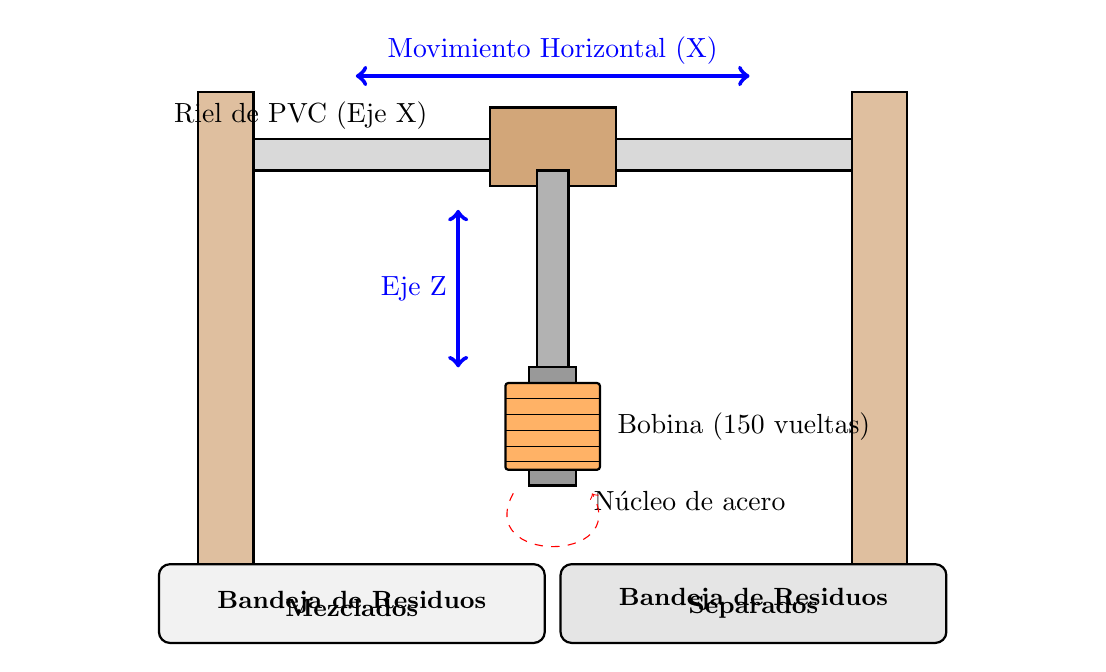
\begin{tikzpicture}[scale=1]
    % Bandeja 1: Residuos Mezclados
    \draw[thick, fill=gray!10, rounded corners] (0,0) rectangle (4.9,1);
    \node[align=center, font=\small\bfseries, text width=8cm] at (2.45,0.5) {Bandeja de Residuos\\[-8pt]Mezclados};

    % Bandeja 2: Residuos Separados
    \draw[thick, fill=gray!20, rounded corners] (5.1,0) rectangle (10,1);
    \node[align=center, font=\small\bfseries, text width=8cm] at (7.55,0.5) {Bandeja de Residuos\\[-8pt]Separados};

    % Columnas de soporte (Madera)
    \draw[thick, fill=brown!50] (0.5, 1) rectangle (1.2, 7);
    \draw[thick, fill=brown!50] (8.8, 1) rectangle (9.5, 7);

    % Riel longitudinal (Tubo PVC)
    \draw[thick, fill=gray!30] (1.2, 6) rectangle (8.8, 6.4);
    \node[above] at (1.8, 6.4) {Riel de PVC (Eje X)};

    % Travesaño móvil (Madera o PVC) con ruedas/deslizador
    \draw[thick, fill=brown!70] (4.2, 5.8) rectangle (5.8, 6.8);
    \draw[<->, ultra thick, blue] (2.5, 7.2) -- (7.5, 7.2) node[midway, above] {Movimiento Horizontal (X)};

    % Mecanismo vertical (Eje Z)
    \draw[thick, fill=gray!60] (4.8, 3.5) rectangle (5.2, 6);
    \draw[<->, ultra thick, blue] (3.8, 3.5) -- (3.8, 5.5) node[midway, left] {Eje Z};

    % Electroimán (Núcleo y Bobina)
    \draw[thick, fill=gray!80] (4.7, 2) rectangle (5.3, 3.5); % Núcleo de hierro
    \draw[thick, fill=orange!60, rounded corners=1pt] (4.4, 2.2) rectangle (5.6, 3.3); % Bobina de cobre

    % Simulación de espiras de alambre
    \foreach \y in {2.3, 2.5, 2.7, 2.9, 3.1}
      \draw (4.4, \y) -- (5.6, \y);

    \node[right] at (5.7, 2.75) {Bobina (150 vueltas)};
    \node[right] at (5.4, 1.8) {Núcleo de acero};

    % Líneas de campo magnético esquemáticas
    \draw[->, dashed, red] (4.5, 1.9) .. controls (4, 1) and (6, 1) .. (5.5, 1.9);
  \end{tikzpicture}%
  }
  \caption{\textit{Plano de elevación frontal del puente grúa manual. Se ilustra el mecanismo de desplazamiento del electroimán en los ejes X y Z sobre las bandejas de separación.}}
  \label{fig:esquema_grua}
\end{figure}

\subsubsection{Fase C: Configuración Experimental y Toma de Datos}
El diseño experimental se basó en la variación de la tensión eléctrica. Se configuró el circuito para operar en cuatro estados utilizando pilas alcalinas en serie (aproximadamente 1.54 V, 3.08 V, 4.62 V y 6.16 V).

Durante las pruebas preliminares, se identificó que la resistencia del alambre variaba rápidamente debido a fluctuaciones térmicas. Por consiguiente, se ajustó el protocolo metodológico: cada lectura de corriente ($I$) se registró estrictamente durante el primer segundo de energización. Posteriormente, el circuito se desconectaba para permitir el enfriamiento de la bobina y evitar el deterioro por Efecto Joule. Las mediciones se realizaron en orden descendente (de 4 a 1 pila) para mitigar el desgaste de la fuente.

A la par, se cuantificó la masa máxima atraída por el electroimán en cada configuración, calculando posteriormente la fuerza de atracción teórica y experimental.

% ==========================================
% RESULTADOS Y DISCUSIÓN
% ==========================================
\section{Resultados y Discusión}

[Espacio reservado para la inserción de las Tablas 1, 2, 3 y 4].

La Figura \ref{fig:graficas_resultados} presenta la evolución del comportamiento electromagnético del prototipo al variar el voltaje de alimentación.

\begin{figure}[H]
  \caption{\textit{Comparación de Datos Teóricos y Experimentales para Fuerza y Campo Magnético según el Voltaje Aplicado}}
  \label{fig:graficas_resultados}
  \centering
  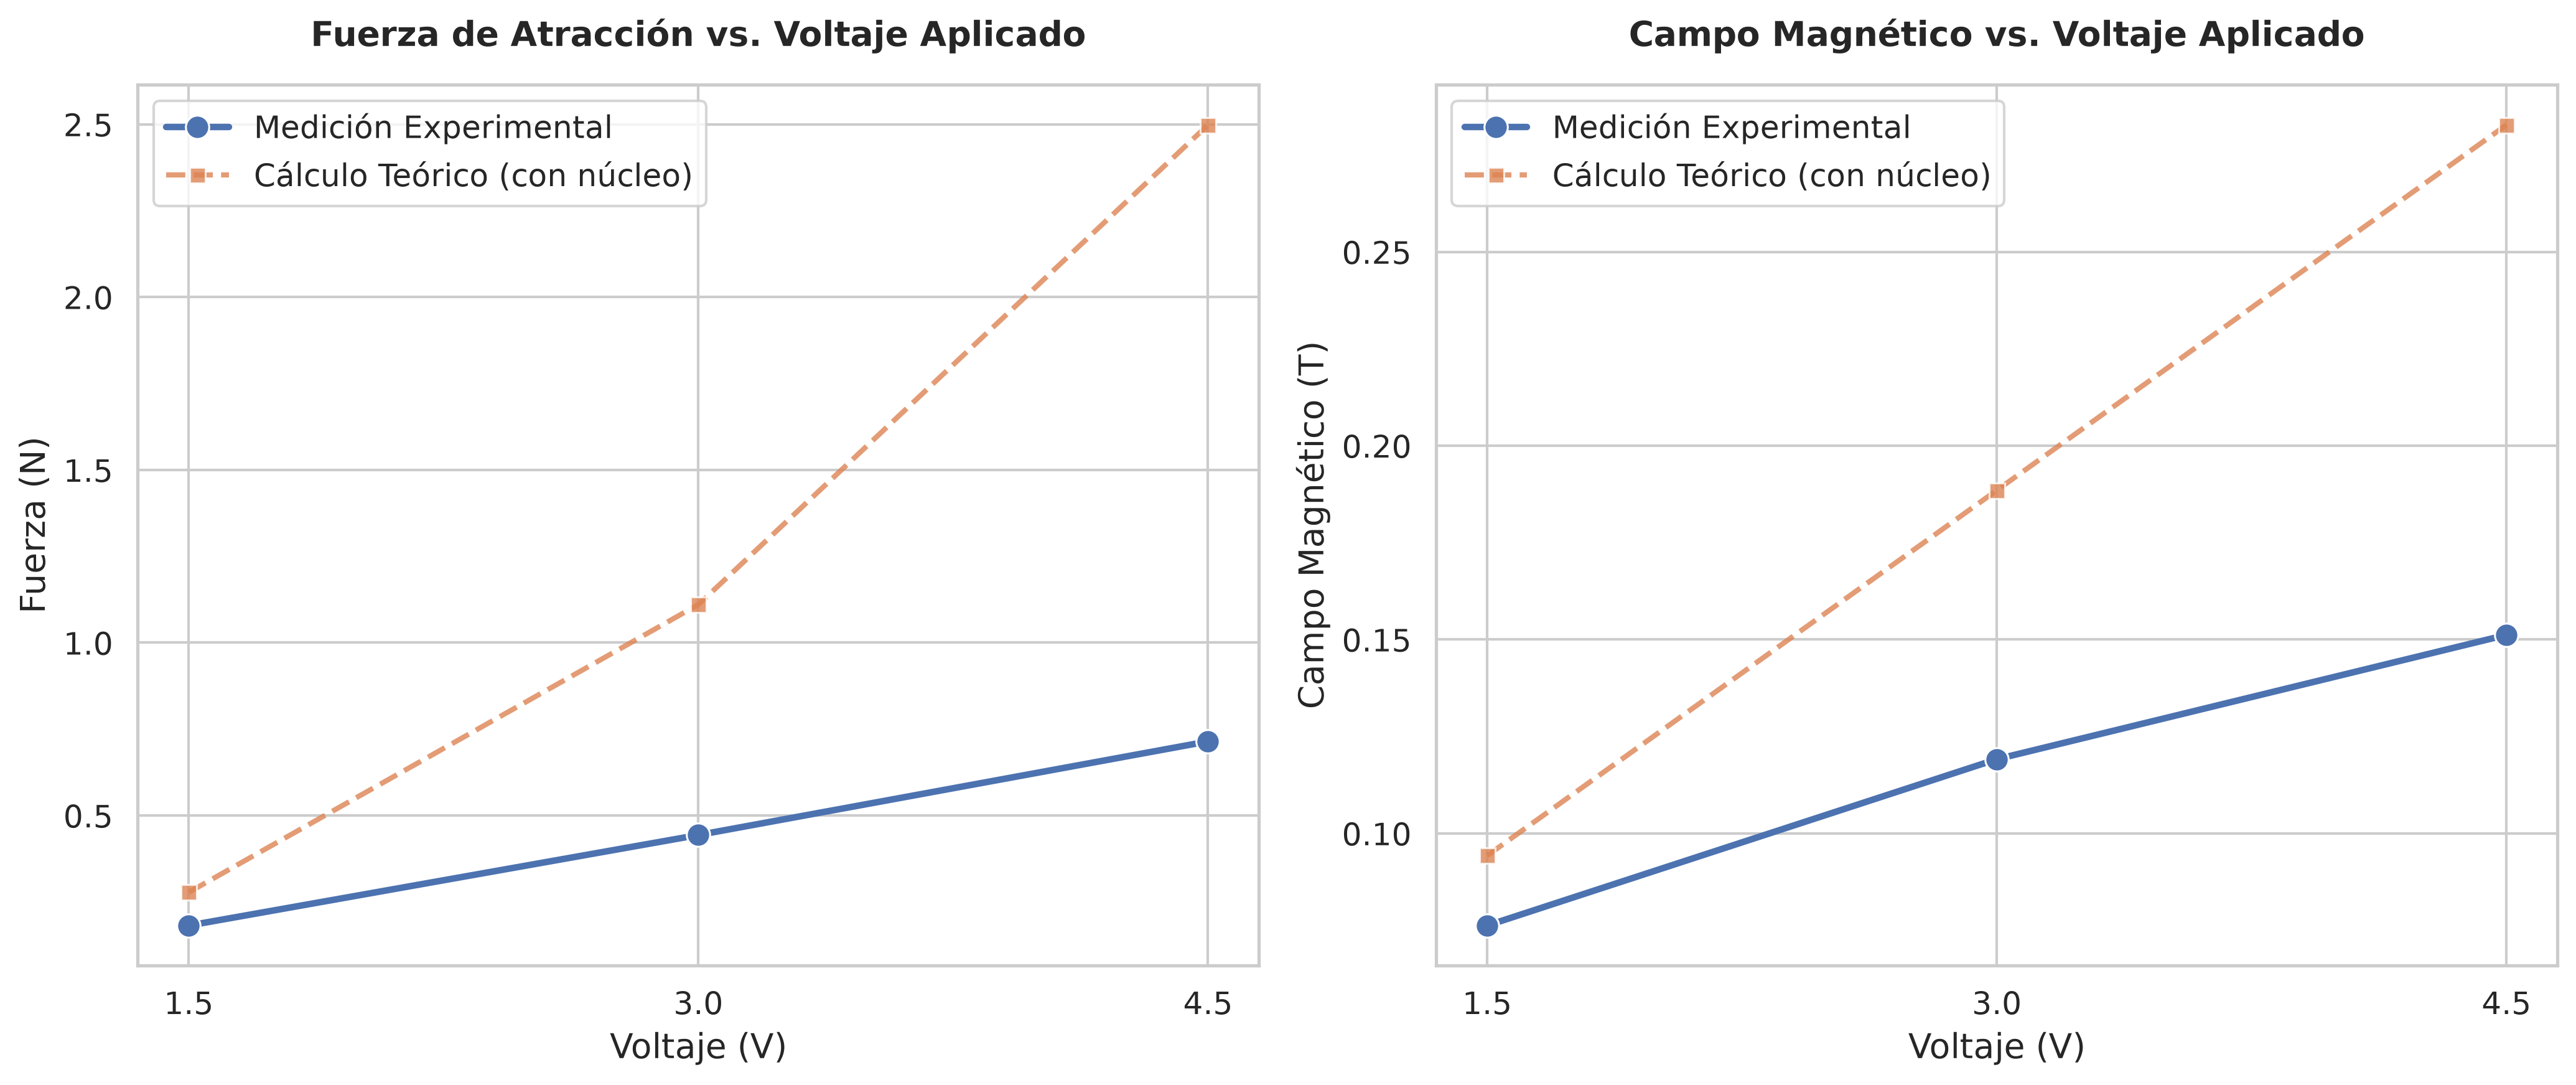
\includegraphics[width=0.9\linewidth]{graficas_resultados.png}
  \begin{figurenotes}
    \textit{Nota.} Las gráficas contrastan los valores experimentales obtenidos en laboratorio frente al modelo teórico ideal.
  \end{figurenotes}
\end{figure}

Como se evidencia en los resultados experimentales, si bien la fuerza de atracción y la corriente eléctrica aumentan a medida que se incrementa el voltaje, existe una clara divergencia no lineal en comparación con el modelo matemático ideal ($I = V/R$). Por ejemplo, la extrapolación teórica para 4 pilas (6.16 V y $0.6 \, \Omega$) predeciría una corriente superior a 10 A; sin embargo, el valor experimental pico registrado fue de 3.19 A. Esta discrepancia obedece a tres fenómenos físicos y técnicos propios de los sistemas reales:

En primer lugar, el modelo ideal asume una fuente de voltaje perfecta. En la realidad, las baterías alcalinas comerciales poseen una resistencia interna inherente. Al exigirles corrientes elevadas, la química interna de la pila se satura, generando una severa caída de tensión en los terminales de salida que actúa como un cuello de botella para el flujo de electrones.

En segundo lugar, se documentó el impacto directo del Efecto Joule. En mediciones iniciales continuas, se observó que el valor de la corriente decaía progresivamente mientras el circuito permanecía cerrado. Esto ocurre porque la disipación térmica eleva rápidamente la temperatura del alambre de cobre, lo que incrementa su resistividad eléctrica ($\rho$) y restringe el paso de la corriente en tiempo real.

Finalmente, las mediciones se ven afectadas por resistencias parásitas introducidas por la instrumentación. Los resortes del portapilas y los cables de prueba del multímetro digital añaden una resistencia adicional al circuito que cobra alta relevancia cuando se operan cargas de muy baja impedancia ($0.6 \, \Omega$), disipando energía en forma de calor antes de que esta alcance el electroimán.

% ==========================================
% APLICACIÓN EN EL ENTORNO
% ==========================================
\section{Aplicación en el Entorno de la Comunidad}
El sistema de puente grúa diseñado a escala modela el funcionamiento de las grúas electromagnéticas utilizadas en los patios de chatarra y centros de acopio municipales. Para una cooperativa local de recicladores, implementar una versión a escala real de este sistema sobre una banda transportadora o en fosas de acopio permitiría separar metales ferrosos (como latas de acero y tapas) de manera rápida y ergonómica. Esto reduce el riesgo de cortes o lesiones en las manos de los operarios y optimiza significativamente el tiempo de clasificación frente a los métodos de separación completamente manuales.
